\chapter{Algorithm HTN}
As discussed in \autoref{chapter2}, % and \autoref{chapter3},
both HTN and Multiagent Planning introduce great interests. But to our knowledge, there is not yet a fully distributed HTN algorithm for multiagent planning. 
In our work, we would finally propose a HTN algorithm for multiagent planning, which is $\emph{by and for}$ a group of agents. But as a first step, we propose a single agent HTN algorithm which is convenient to extend to multiagent situation. In this chapter, firstly, we introduce the basic idea of our HTN planner; then we give some detailed definitions corresponding to our planner; finally, we propose, explain and discuss our algorithm.
%
%As mentioned in \autoref{chapter3}, we would finally propose a HTN algorithm for multiagent planning. But as a first step, we propose a single agent HTN algorithm which is convenient to extend to multiagent situation. In this chapter, firstly, we introduce the basic idea of our HTN planner; then we give some detailed definitions corresponding to our planner; finally, we propose, explain and discuss our algorithm.

\section{Basic Idea}
One of the interests of multiagent planning is the distributed planning process. But for HTN algorithms like SHOP (explained in \autoref{sec:SHOP}), it is difficult to distribute the planning process to a group of agents, since it plans from the first task to the last one, it needs exact world state in each step to verify constraints and methods’ preconditions. In another word, the planning process of SHOP is inherently a sequential process, the tasks must be planned one by one, a plan can not be refined by several agents in parallel.

To the contrary, UMCP (explained in \autoref{sec:UMCP}) does not need exact world state, it refines compound task without caring about tasks’ order. To verify the constraints, during its planning process, some constraints are considered as promises, since there is not yet enough information to verify it, a promissory constraint can only be verified until some necessary compound tasks are refined.

For being extended to multiagent planner in the future, our planner has been based on UMCP. We have chosen UMCP for the following reasons:
\begin{itemize}
\item[-] As discussed above, for a planner like SHOP, it is almost impossible to allocate tasks to a group of agents.%, its forward searching feature causes difficulty in the phase “Goal and task allocation” (as explained in \autoref{phases_multi}). 
Differently, UMCP has no limit on tasks’ planning order, this feature makes a multiagent planner much more powerful and flexible. It gives the possibility that a group of agents work on the same HTN (i.e. to divide a HTN into several parts, each agent plans its own part).
\item[-] The planners like SHOP produce totally-ordered plan, which is not convenient for a group of agents’ execution (i.e. a totally-ordered plan forces too much wait in MAS, there can be only one agent executing an action at a time). On the contrary, UMCP produces partially-ordered plan, the actions between which there is no ordering constraint can be executed in parallel.
%\item[]
\end{itemize}

\section{Definitions}

Some definitions for our algorithm are as follows:
\begin{definition}[Task]
A task symbol is the name of a primitive task or a compound task. 
A task consists of a task symbol and its arguments (i.e. a list of objects).
\end{definition}

% There is a special compound task $\emph{achieve(p)}$, its argument $\emph{p}$ is a predicate, the task aims at achieving $\emph{p}$. So its refinement is with an after constraint like ($t_{last}$,p) to guarantee that after its execution, $\emph{p}$ is satisfied, $t_{last}$ is the last task in its refinement.

\begin{definition}[Actions/Operators]
An operator is an expression of the form ($:$operator $\emph{t, P, E}$) where $\emph{t}$ is a primitive task, $\emph{P}$ is the precondition of $\emph{t}$, $\emph{E}$ is the effect.
\end{definition}

\begin{definition}[Method]
A method is an expression of the form ($:$method $\emph{h, P, d}$) where $\emph{h}$ is the method's corresponding compound task, $\emph{P}$ is the precondition of the method, $\emph{d}$ is the HTN to refine to when applying this method.
\end{definition}

\begin{definition}[Planning Domain]
A planning domain in our algorithm is a tuple ($\emph{O, M}$) where $\emph{O}$ is the set of operators and $\emph{M}$ is the set of methods.
\end{definition}


\begin{definition}[Planning Problem]
A planning problem in our algorithm is a tuple ($\emph{d, I, D}$) where $\emph{d}$ is the initial HTN, $\emph{I}$ is the initial state, $\emph{D}$ is the planning domain.
\end{definition}


\begin{definition}[Linearization]
A linearization of a partially-ordered plan is a totally-ordered plan which satisfies all the ordering constraints of the partially-ordered plan.
\end{definition}

For example, the plan in \autoref{fig4_1} has two linearizations:
\begin{itemize}
\item[] $\emph{A}$ $\prec$ $\emph{B}$ $\prec$ $\emph{C}$
\item[] $\emph{A}$ $\prec$ $\emph{C}$ $\prec$ $\emph{B}$
\end{itemize}

\begin{figure}[H]
    \center
    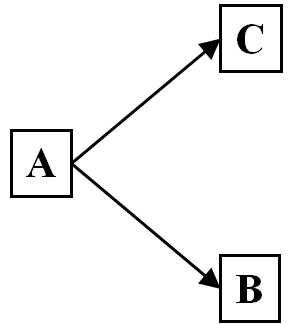
\includegraphics[width=0.2\textwidth]{./images/4_1.png}
    \caption{A partially-ordered plan}
    \label{fig4_1}
\end{figure}

\begin{definition}[Solution Plan]
A solution plan is a partially-ordered plan, each of its linearizations satisfies all the state constraints of the plan.
\end{definition}

\section{Planning Algorithm}
Our algorithm is as follows:

\begin{algorithm}[H] 
\caption{HTN Planning Algorithm}
\label{algo1}
\KwIn{a planning problem $=$ <d, I, D>} 
\KwOut{solution plan}
\\[0.2cm]
\If{CheckOrderCircle(d)} { 
	return FAIL;
}\\[0.2cm]

openList $\leftarrow$ d;\\
solution $\leftarrow$ FAIL;\\[0.2cm]

\While{ openList $\ne$ $\emptyset$ $\wedge$ solution $=$ NULL } {
	p $\leftarrow$ PopBestPlan(openList);\\
	t $\leftarrow$ SelectBestTask(p);\\[0.2cm]

	\If{t $=$ NULL $\wedge$ IsConstrSatisfied(p) $=$ TRUE } { 
		solution $\leftarrow$ p;
	}\\[0.2cm]

	\If{t\ $\ne$ NULL } {
		\For{ each m $\in$ GetRelevantMethods(t,D) }
		{
			newPlan $\leftarrow$ Refine(t, m, p);\\
			openList $\leftarrow$ openList $\bigcup$ newPlan;
		}
	}
}\\[0.2cm]

return solution;
\end{algorithm}

In line 1-2, we check if the input plan contains any ordering circle. If a circle exists, there is no need to search, we return FAIL directly (as explained in \autoref{sec:constraints}). Here only the input HTN is checked, the refinements within methods should be checked before the planning (i.e. right after parsing), so they are assumed to contain no circle when the planning begins. If neither the input HTN nor the methods contain any ordering circle, we will never obtain a circle through refining.

In line 3-4, the variable $\emph{openList}$ is initialized to contain only the initial HTN $\emph{d}$. The variable $\emph{solution}$ is for storing the solution plan, it is initialized as FAIL.

In line 5, the algorithm checks whether $\emph{openList}$ is empty or a solution plan has been found, if so, the planning loop stops; if not, the loop continues.

In line 6, the function $\emph{PopBestPlan}$ implements a heuristic which pops a plan $\emph{p}$ (i.e. a plan is a HTN) from $\emph{openList}$, the popped plan should be the one which is the most likely to be a solution. The heuristics will be explained in \autoref{chapter_heuristic}.

In line 7, the function $\emph{SelectBestTask}$ implements another heuristic on the compound tasks, it returns a compound task $\emph{t}$ to refine. If the popped plan $\emph{p}$ is already primitive (i.e. $\emph{p}$ contains no compound task), the function $\emph{SelectBestTask}$ returns NULL. The heuristics will be explained in \autoref{chapter_heuristic}.

in line 8-9, if $\emph{t}$ is NULL, the function $\emph{IsConstrSatisfied}$ will be called, it checks if all the state constraints of $\emph{p}$ have been satisfied. Since initial state $\emph{I}$ and effects of primitive tasks are input, the plan $\emph{p}$ is primitive, obviously, all the world states are certain, we have been able to verify all the state constraints. If $\emph{p}$ is indeed a solution (i.e. $\emph{p}$ is primitive and all the constraints are satisfied), $\emph{p}$ will be assigned to $\emph{solution}$.  

In line 10, if $\emph{t}$ is not NULL (i.e. $\emph{p}$ contains at least one compound task), the algorithm will enter into the following loop to refine $\emph{t}$.

In line 11, the function $\emph{GetRelevantMethods}$ returns all the  methods whose associated compound task is $\emph{t}$, then each of these methods will be applied.

In line 12, the function $\emph{Refine}$ is called, it applies method $\emph{m}$ for refining task $\emph{t}$, a new HTN is obtained, the variable $\emph{newPlan}$ stores the newly obtained plan. The details of function $\emph{Refine}$ will be discussed in the next section.

In line 13, $\emph{openList}$ is updated to contain the newly obtained HTN $\emph{newPlan}$.

\section{Refining Algorithm}
The algorithm of the function $\emph{Refine}$ is as follows:

\begin{algorithm}[H] 
\caption{Refining Algorithm} 
\KwIn{Task: t, Method: m, Plan: p} 
\KwOut{newPlan}
\\[0.2cm]
newPlan $\leftarrow$ p;\\
refinement $\leftarrow$ GetRefinement(m, t);\\
precond $\leftarrow$ GetPrecond(m, t);\\[0.2cm]

MergeConstr(newPlan, precond, t);\\
\If{IsConstrUnsatisfiable(precond, t, newPlan) } {
    return $\emptyset$;
}\\[0.2cm]

MergePlan(newPlan, refinement);\\
TransferConstr(newPlan, t);\\
RemoveTask(newPlan, t);\\[0.2cm]

VerifyAllConstr(newPlan);\\
\If{IsConstrUnsatisfiable(newPlan) } {
    return $\emptyset$;
}\\[0.2cm]

return newPlan;
\end{algorithm}

The input of the Refining Algorithm includes:
\begin{itemize}
\item[] \textbf{t}: the task to refine (the task obtained in line 8 of Algorithm 1, as in page \pageref{algo1});
\item[] \textbf{m}: the method to apply (as in line 13,14 of Algorithm 1);
\item[] \textbf{p}: the original plan (the plan obtained in line 7 of Algorithm 1).
%\item[] 
\end{itemize}

In line 1, the variable $\emph{newPlan}$ is initialized as a copy of the input plan $\emph{p}$. 

In line 2, the function $\emph{GetRefinement(m, t)}$ returns the compound task $\emph{t}$’s refinement (i.e. an instance of $\emph{m}$’s associated refinement).

In line 3, The function $\emph{GetPrecond(m, t)}$ returns the precondition of $\emph{m}$ for refining $\emph{t}$ (i.e. an instance of $\emph{m}$’s precondition). 

In line 4, $\emph{precond}$ is converted to a before constraint ($\emph{precond}$,$\emph{t}$), and it is merged into $\emph{newPlan}$.

In line 5-6, we check if the before constraint ($\emph{precond}$,$\emph{t}$) is unsatisfiable(i.e. the constraint can never get satisfied), if so, the method $\emph{m}$ is not applicable, and there is no need to continue the refining, the algorithm returns an empty set $\emptyset$.

In line 7, the HTN $\emph{refinement}$ is merged into the HTN $\emph{newPlan}$. If two HTNs $p_1 = ((n_1: a_1) \ldots (n_i: a_i), C_1)$, $p_2 = ((n_1: b_1) \ldots (n_i: b_i), C_2)$. After $MergePlan(p_1, p_2)$, $p_1 = ((n_1: a_1) \ldots (n_i: a_i) (n_{i+1}: b_1) \ldots (n_{i+j}: b_j), C_3)$, where $C_3 = C_1 \cup C_2'$.

The constraints (i.e. both ordering constraints and state constraints) of $C_2$ can not be merged into $\emph{newPlan}$ directly. The labels within constraints of $C_2$ must be updated before merging (A string label is much more memory-consuming than an integer label in the data structure of the algorithm, so here we do not discuss updating the part “n” of a label $n_i$). A label $n_k (k \in [1, j])$ should be updated as $n_{i+k}$. Then $C_2'$ (the updated $C_2$) is added in $C_1$ without violating the mapping between labels and tasks. Through merging, we add all the information in the compound task’s refinement into the original plan.

In line 8, before removing $\emph{t}$, we must transfer constraints on $\emph{t}$ to the corresponding constraints on $\emph{t}$’s refinement, and add the newly obtained constraints in $\emph{newPlan}$. If $\emph{p}$ is a predicate, compound task $\emph{t}$’s label is $n_t$ in $\emph{newPlan}$, the updated labels and their corresponding tasks of $\emph{refinement}$ are ($(n_{i+1}: b_1) \ldots (n_{i+j}: b_j)$). All kinds of concerned constraints and their replacements are as follows, the item before “$\rightarrow$” is the constraint to be replaced, the one after is its replacement. (the semantics of $\emph{first}$ and $\emph{last}$ are explained in \autoref{sec:constraints})

\begin{itemize}
\item[$\bullet$] \textbf{After constraint} ($n_t$, p) $\rightarrow$ (last[$n_{i+1},\ldots ,n_{i+j}$], p)
\item[$\bullet$] \textbf{Before constraint} (p, $n_t$) $\rightarrow$ (p, first[$n_{i+1},\ldots ,n_{i+j}$])
\item[$\bullet$] \textbf{Between constraint} 
    \begin{itemize}
    \item[-] ($n_i, p, n_t$) $\rightarrow$ ($n_i$, p, first[$n_{i+1},\ldots ,n_{i+j}$])
    \item[-] ($n_t, p, n_i$) $\rightarrow$ (last[$n_{i+1},\ldots ,n_{i+j}$], p, $n_i$)
    \end{itemize}
\item[$\bullet$] \textbf{Ordering constraint}
    \begin{itemize}
    \item[-] ($n_i \prec n_t$) $\rightarrow$ ($n_i \prec$ first[$n_{i+1},\ldots ,n_{i+j}$])
    \item[-] ($n_t \prec n_i$) $\rightarrow$ (last[$n_{i+1},\ldots ,n_{i+j}$] $\prec n_i$)
    %\item[]
    \end{itemize}
\end{itemize}

If the refinement of $\emph{t}$ is empty (i.e. $\emph{refinement} =$ NULL), the replacement of the concerned constraints will be NULL. Through  constraints’ transfer, we guarantee to refine without violating the original constraints.

In line 9, the task $\emph{t}$ is removed from the HTN $\emph{newPlan}$, all the constraints which contain the label of $\emph{t}$ will also be removed.

In line 10, all the constraints of $\emph{newPlan}$ are verified. In $\emph{newPlan}$, the sets of $\emph{verified constraints}$, $\emph{promissory constraints}$ and $\emph{unsatisfiable constraints}$ are updated. A constraint is verified only if it is satisfied in every linearization of the plan. On the contrary, a constraint is unsatisfiable if there exists any linearization in which the constraint is unsatisfiable; it’s the same for promissory constraint, even if a constraint is satisfied in all the linearization except one in which it is promissory, then it is a promissory constraint.

In line 11-13, if the performed refining causes a $\emph{unsatisfiable constraint}$ (i.e. there exists a $\emph{unsatisfiable constraint}$ in $\emph{newPlan}$), the algorithm returns $\emptyset$. If not, it returns $\emph{newPlan}$. The returned plan is added in $\emph{openList}$ in line 15 of Algorithm 1 (as in page \pageref{algo1}).

\section{Our Algorithm vs UMCP}
Our algorithm shares the same basic idea with UMCP, but there still exists some differences:

\begin{itemize}
\item[-] In our algorithm, we use $\emph{openList}$ to store all the plans which possibly lead to a solution. This allows us to implement a heuristic to improve the search efficiency. In UMCP, the search is nondeterministic.
\item[-] In our algorithm, all relevant methods of a compound task are applied when refining it, and all obtained plans are added in $\emph{openList}$. In another word, all possibilities are considered when refining, so there will not be any backtrack. Differently, in UMCP, a backtrack is necessary when the search reaches a dead end. The backtrack causes many difficulties, not only on the choice of node (i.e. task) to backtrack to, but also on avoiding choosing an applied method.
\item[-] We have not applied $\emph{critics}$ which is used in UMCP. $\emph{critics}$ repairs flaws caused by interaction of tasks, or it refuses the plan if a flaw can not be repaired. UMCP considers only a single plan during search, which makes the correctness of the current plan important. Differently, in our algorithm, a group of plans are considered, which makes applying $\emph{critics}$ not so meaningful to us.
\end{itemize}
